\section{The first negative second difference}
\label{sec:first-change}

\begin{theorem}\label{thm:firstchange}
For the Riemann Li coefficients,
\[
 d_j>0.00014\quad (0\le j\le117),\qquad d_{118}<-0.00026.
\]
Thus the first negative centered second difference occurs at $j=118$.
For a set of positive lower Banach density of $k$, each of the two
centers $k^2$ and $k^3$ lies at the middle of a maximal run of exactly
235 positive second differences, immediately preceded and followed by
negative values. Both runs have the same strict bounds as above.
The same assertion holds at the two centers $(p-1)^2$ and $(p-1)^3$
for a set of primes $p$ of positive lower relative density.
\end{theorem}

\begin{proof}
For the forty positive ordinates certified in Section~\ref{sec:signs}
write $w_j=w(t_j)$ and $\theta_j=\theta(t_j)$, with the definitions
used there. For any phase angle $\theta$ set $x=1-\cos\theta$.
Let $M_i$ be the total mass of $x^i$ in the spectral measure from
\eqref{eq:fourier}, and $r_i$ its mass after deleting these forty pairs.
The double-angle identity gives
\[
 M_0=C,\qquad M_1=C-d_1,\qquad
 M_2=\frac{3C-4d_1+d_2}{2}.
\]
Write \(L=\log\xi\) near \(1\). The formulas in Section~\ref{sec:windows}, together with
\[
 L'''(1)=2-\tfrac74\zeta(3)+3\gamma_2+6\gamma\gamma_1+2\gamma^3,\qquad
 \lambda_3=3L'(1)+3L''(1)+\tfrac12 L'''(1),
\]
give all three moments. The identities follow by taking the next term in the Laurent expansion, \((s-1)\zeta(s)=1+\gamma(s-1)-\gamma_1(s-1)^2+\gamma_2(s-1)^3/2+\cdots\), and differentiating the gamma factor. In particular,
\[
 \frac{718389301443}{10^{19}}\le M_2\le
 \frac{718389301444}{10^{19}}.
\]
For a pair, $x_j=1/(2(1/4+t_j^2))=w_j/4$, so the omitted moments are
$r_i=M_i-\sum_{j=1}^{40} w_j(w_j/4)^i$.

For $0\le x\le2$ and $n\ge0$, the Chebyshev polynomial satisfies
\begin{equation}
 1-n^2x\ \le T_n(1-x)\le
 1-n^2x+\frac{n^2(n^2-1)}{6}\,x^2.\label{eq:quadratic-tail}
\end{equation}
Indeed, $|T_n'|\le n^2$ on $[-1,1]$ follows from
$|\sin(n\theta)|\le n|\sin\theta|$. The identity
$T_n'=n\sum_{j=0}^{n-1}T_{|n-1-2j|}$ then gives
\[
 \max_{[-1,1]}|T_n''|\le n\sum_{j=0}^{n-1}(n-1-2j)^2
 =\frac{n^2(n^2-1)}3.
\]
The mean value theorem gives the lower bound in
\eqref{eq:quadratic-tail}, and Taylor's theorem at $1$ gives the upper
bound, including the linear coefficient $T'_n(1)=n^2$. The constant
case $n=0$ is immediate.

Put $S_n=\sum_{j=1}^{40}w_j\cos(n\theta_j)$. Summing
\eqref{eq:quadratic-tail} against the omitted positive measure gives
\[
 S_n+r_0-n^2r_1\le d_n\le
 S_n+r_0-n^2r_1+\frac{n^2(n^2-1)}6\,r_2.
\]
The script \texttt{certify\_window.py} checks the displayed
inequalities in the theorem at all 119 indices, including
\begin{align*}
 0.000147247112&\le d_{117}\le\phantom{-}0.000201258543,\\
 -0.000325756767&\le d_{118}\le-0.000269874914.
\end{align*}
Figure~\ref{fig:window} plots all the enclosures. The accompanying CSV gives the outward-rounded rational endpoints. The moment script evaluates $(\log\xi)^{(i)}(1)$, $i=1,2,3$,
from $\gamma,\gamma_1,\gamma_2,\pi$ and $\zeta(3)$ by
Euler--Maclaurin summation and rational intervals.

Finally $d_{-j}=d_j$, so the bilateral sequence has a run of $235$
positive terms on $[-117,117]$, bracketed by two negatives.
Take a uniform recurrence tolerance below the least of the strict
margins in this finite pattern. Theorem~\ref{thm:curv} with
$k^2,k^3$ transfers every sign and bound to both translated
patterns. In the prime case the two displayed polynomials have a
common unit root $1$ modulo every integer.
\end{proof}

\paragraph{Independent verification by a Taylor series.}
The finite calculation also follows directly from Johansson's power-series method \cite{joh}, independently of the zero-location theorem. Set \(s=-z/(1-z)\). The functional equation gives
\(\log(2\xi(s))=\log2+L(1+z/(1-z))\) near \(z=0\). For \(n\ge1\) the degree-\(n\) coefficient is
\[
 \sum_{j=1}^n \binom{n-1}{j-1}\frac{L^{(j)}(1)}{j!}=\lambda_n/n
\]
by Li's derivative formula and the product rule. The script \texttt{verify\_keiper.py} evaluates
\[
 \log(1-s)+\log(-2\zeta(s))-\tfrac{s}{2}\log\pi+\log\Gamma(1+s/2)
\]
through degree 119 using 512-bit Arb ball arithmetic. It certifies all 119 comparisons directly, with \(d_{117}=0.000200146986527119643036209\) and \(d_{118}=-0.000271044467116152907821086\), each to within \(5\cdot10^{-28}\).

\begin{figure}[htbp]
\centering
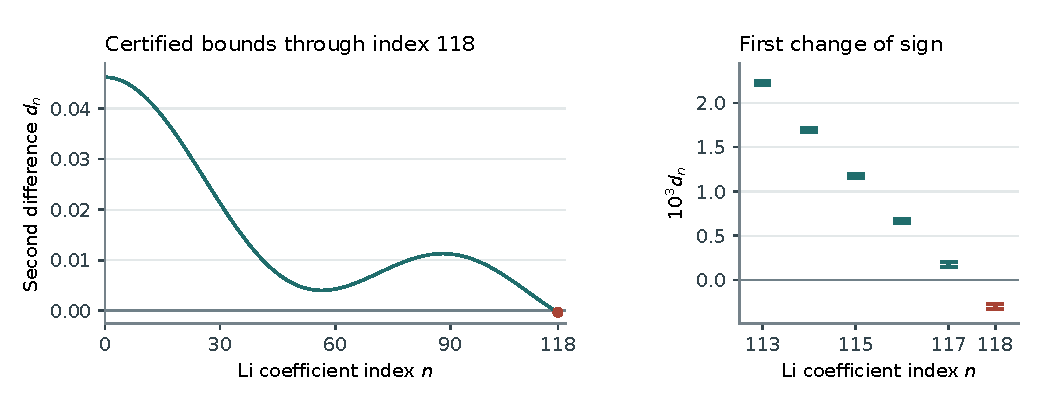
\includegraphics[width=.96\linewidth]{curvature_bounds.pdf}
\caption{Certified intervals for the centered second differences \(d_n\).
At full scale many intervals are thinner than the line. The right panel
shows the bounds on each integer separately, on an enlarged vertical scale.}
\label{fig:window}
\end{figure}
